
\documentclass[msc,ai,logo,sansheadings]{infthesis}
\shieldtype{3}

\usepackage{natbib}
\usepackage{graphicx}
\usepackage{listings}
\usepackage[english]{babel}

\title{Paraphrasing In The Context Of \\ Computer Aided Translation}
\author{Turan Rustamli}

\abstract{%
    ...
}


\begin{document}

\begin{preliminary}

\maketitle

\begin{acknowledgements}
...
\end{acknowledgements}

\standarddeclaration

%% \dedication{To my mummy.}

\tableofcontents

% \listoffigures
% \listoftables

\end{preliminary}

%%%%%%%%
%% Include your chapter files here. See the sample chapter file for the basic
%% format.

\chapter{Introduction}
  
\section{Motivation}

Today by taking advantage of achievements in machine translation, we can read and understand text in languages unknown to us. However, high quality translation still needs involvement of human translators. Computer Aided Translation (CAT) aims to support and assist translators, providing them with tools that partially automate and simplify their workflow. Demand for these tools is huge, each year international organisations such as European Union spend billions on translation services. 

Over past years researchers introduced several ways to aid translators. The most popular ones are interactive machine translation and post-editing. The first approach provides translation suggestions as user types, while the second approach initiates input area with a machine translation. 

During current project we developed and evaluated a novel assistance way that aims to help translators to improve a machine translation, by paraphrasing any part of the sentence that they specify.

Paraphrasing is a process of representing the same idea with different words. Some recent publications suggest that the paraphrasing and the translation tasks are closely related. Moreover, information used to perform one task, can be useful for another \citep{Callison-Burch2007}. 

In this report we will introduce a paraphrasing approach that efficiently reuses outcomes of the machine translation process. Also, we will describe how paraphrasing performance can be improved within an interactive translation environment, by considering user feedback on the results. Finally, we will present a novel automatic evaluation approach that we used to test feasibility and usefulness of our paraphrasing tool. To confirm the automatic evaluation results we carried out several user studies. We will share outcomes of these experiments and discuss how they correlate with our previous findings. 

\section{Overview}

In this section we provide an outline of the report. We will start Chapter 2 by introducing background material that aims to provide required information about the context of our project. We will describe recent advancements in Computer Aided Translation and relate existing assistance tools to our paraphrasing service. Next we will provide references to previous publications on paraphrasing. We will also discuss some basic concepts of machine translation, focusing on the decoding process. The data structure generated during this process is known as search graph and it is used by us as the main source for paraphrasing. 

In Chapter 3 we will describe the work that was carried out in scope of current project. Firstly, we will start by discussing the design of our approach and possible ways of integration with existing CAT tools. We will continue by providing implementation details for each component of our initial design. In this chapter we will also focus on challenging problems that were discovered during design and implementation stages, and their solutions.

We will present our evaluation methodology in Chapter 4. We will provide description of an automatic evaluation process which was carried out by us during the project. Furthermore, we will presents evaluation results for ten different versions of our paraphrasing algorithm. We will continue by discussing advantages and disadvantages of the automatic evaluation. Finally, we will provide results of user studies that confirm our previous results.

In Chapter 5 we will present an improved paraphrasing approach that responds to user feedback in order to provide more relevant results. We will also describe a modification that we applied to our automatic evaluation tool in order to support this new feature. We will finish this chapter by introducing another interactive feature, that lets users to make specified paraphrasing requests.  

Finally, in Chapter 6 we will conclude our report and suggest interesting directions for future work. 

\chapter{Background}


The main goal of our project was providing a paraphrasing service within a Computer Aided Translation system by reusing the result of the machine translation process, which is used to provide other types of assistance. Before introducing our approach, we would like to provide some background information about assistance types available within CAT systems, existing paraphrasing approaches and some basic concepts of machine translation.

\section{Computer Aided Translation}

Recently, more and more papers discussing various aspects of Computer Aided Translation are published. This increase can be explained by the fact that efficient usage of machine translation advancements to increase productivity of translators is still an open problem. Various assistance tools have been suggested and implemented. Most of these tools are reportedly increasing translation speed, others help to achieve better quality. In this work we present a novel assistance type, which aims to help translators by providing a paraphrasing service. Therefore we want to start by highlighting how our approach could be used in the context of CAT systems together with other assistance types.

\subsection{Interactive Machine Translation}

One way to assist translators is providing auto-completion suggestions while the translation in target language is being composed. As user input in text editor component changes, system suggests possible translation of the next word or phrase. The first system implementing this approach was \emph{TransType} \citep{langlais2000transtype}. TransType is providing optional sentence-completion suggestions based on machine translation. Considering user acceptance of the suggestions, system can be improved to provide better results \citep{barrachina2009statistical}. \emph{Caitra} is another CAT system described by \cite{KoehnHaddow2009}, which also provides an interactive mode. 

Our paraphrasing approach similarly reuses the search graph to generate paraphrasing options, however in contrast to Interactive Machine Translation systems we assume that the user already has an initial translation that needs to be improved. This initial translation could be originally produced using an interactive assistance with auto-completion or, alternatively, it could be an automatic translation provided for post-editing.

\subsection{Post-Editing}

Popular type of assistance is providing machine translation output as initial translation that could be edited by translator. In this case for each sentence in the document that is being translated, the system provides multiple translation versions. The user can select one of these versions and edit it in order to achieve a high quality translation. Alternatively, the user can ignore suggested options and start typing the translation manually and possibly taking advantage of an aforementioned interactive suggestion tool.  

The effect of post-editing on productivity of the translators was analysed by many researchers, including \cite{guerberof2009productivity}. It was previously demonstrated that post-editing can significantly improve performance of translator in some contexts like legal and information technology documents \citep{federico2012measuring}. However, in other domains like news and media, initial translations produced for post-editing are far from publishable quality. This output is being manually fixed and improved, by replacing erroneous parts with correct words preserving the meaning. This is one of the situations when our paraphrasing service can help user to find better ways to express the ideas in the corrupted parts.

Our current implementation of the paraphrasing tool can be integrated only with a CAT system that provides post-editing assistance. However our approach requires only information generated during machine translation decoding. Considering this, our service can be easily extended to be used with the CAT systems that provide machine translation driven assistance by other means.

\subsection{Bilingual concordancer}

A bilingual concordancer is a feature used by professional translators to explore alternative translations of particular source language phrases. This is achieved by finding occurrences of the phrase in a bilingual corpus and retrieving their corresponding translations. Analysing usage logs of \emph{TransSearch}, one of the most popular bilingual concordancers, for 6 years demonstrate that tranlators find this feature useful especially for finding the correct sense in case of highly polysemous adverbials and prepositional phrases \citep{Macklovitch2008}. Our tool in contrast, is supposed to work with target language words. Given one possible translation of a phrase, it finds other alternative translations. Similarly, to bilingual concordancer, this might be useful for finding a translation that preserves the meaning of the original phrase in a better way. We expect that starting a search for alternative translations within the same language, will simplify the this task for users with poor understanding of the source language.

\subsection{Other assistance ways}

Providing various translation options for parts of sentence in the source language, can also help in the translation task. As it was shown by \cite{Koehn2010}, using this assistance enables translation with acceptable quality even without understanding the source language. The difference of our approach is that instead of providing different translation options for all parts of the original text, we produce paraphrasing suggestions for a user specified parts of translation. Thus similarly to translation options, our tool can be used by someone, who doesn't know source language. For example it may help to understand unclear parts of the text provided for post-editing, by paraphrasing them into representations that make more sense.

Finally, feasibility of our approach could be improved when used together with other CAT features like idioms and terminology detections. Indeed, if idioms or terminology are marked up in user input, during paraphrasing they can be treated in specific ways. In case of terminology paraphrasing lookup might take benefits of domain specific thesauruses. For idioms the paraphrasing algorithm will consider them as atomic units and will not try to paraphrase them partially. 

\subsection{Summary}

In this section, we described how our paraphrasing service could be used together with other assistance types within a CAT system. While our implementation requires data generated by a machine translation decoder, this data is not supposed to be generated separately specifically for paraphrasing needs. The data available after running a translation system for an interactive assistance or post-editing could be successfully reused for paraphrasing needs. We also compared our approach with tools like a bilingual concordancer and translation options, highlighting similarities and differences. And finally, we mentioned how paraphrasing could take advantage of idiom and terminology detectors.

\section{Paraphrasing Approaches}

Here we will summarise outcomes of a variety of data-driven paraphrasing techniques previously available in the literature. We want to acknowledge that essential difference of our approach from the ones listed in this section is that while most of previous studies were focused on paraphrasing generation problem, our approach is considering paraphrasing as a search problem. Paraphrasing generation aims to different find ways of extracting paraphrases from various sources and store them for future usage. Paraphrasing search aims to find paraphrases for a specific phrase that is given in a context of a specific sentence that is being translated by a user. Despite this difference ideas from these approaches were used by us for achieving better results and for developing an automatic evaluation approach that was used to assess multiple versions of our paraphrasing algorithm. In this section we will mainly focus on data-driven paraphrasing approaches reviewed in \cite{Callison-Burch2007}. 

\subsection{Data-driven paraphrasing}

Originally paraphrasing was considered within multiple problems in Natural Language Processing, including question answering, summarisation and natural language generation. As a result historically there were multiple approaches for paraphrasing including techniques that use formal semantic representation and methods that use grammars. More recent approaches are statistically motivated and make use of various data sources to generate paraphrases. 
Main data sources that were previously used in literature include multiple translations, comparable corpora and monolingual corpora. A novel technique introduced by \cite{Callison-Burch2007}, describes how bilingual parallel corpora could be used for paraphrase generation, this approach is related to the technique we use for paraphrasing. Similarly, the data we exploit is built during a statistical machine translation process and derives from a bilingual parallel corpus.

\subsection{Multiple translations}

The key idea of the techniques that exploit multiple translations as a data source for paraphrase generation is that translators composing different translations of the same text preserve its original meaning, what makes these translations natural sources for paraphrasing \citep{barzilay2001extracting}. The first experiments with multiple translation of French classical literature were focused on extracting paraphrases by detecting different phrases in similar contexts. So for example, following French sentence, might be translated into English in two different ways as follows:

\begin{center}
\begin{Large}
\textbf{G\`{e}n\`{e}ralement, les gens qui savant peu parlent becoup,\\ et les gens qui savant beaucoup parlent peu}
\\
\small{\textit{(Jean-Jacques Rousseau)}}
\end{Large}
\end{center}

\begin{center}
\begin{Large}
People who know little speak a lot, and the people who know a lot speak little. 
\end{Large}
\end{center}

\begin{center}
\begin{Large}
People who know little are usually great talkers, while men who know much say little.
\end{Large}
\end{center}

Aligning similar parts of both sentences, we can see that ``are usually great talkers'' and ``speak a lot'' appear in same context and therefore they probably have same meaning.

Later researchers applied more complex ways to detect paraphrases in multiple translations, this includes using parse trees and considering parts of sentence with similar syntactic role to be paraphrases \citep{pang2003syntax}.

While our paraphrasing approach does not exploit these ideas, we used similar technique to generate test cases for automatic paraphrasing evaluation. Instead of multiple translations that are rarely available, we used a machine translation to corrupt natural language sentences, and later used difference between original and corrupted sentences as a test case. This technique similarly decides whether parts represent the same idea by considering the surrounding context. Our evaluation methodology will be discussed in detail in Chapter 4.

\subsection{Bilingual parallel corpus}

Close ties between paraphrasing and translation were studied by \cite{Callison-Burch2007}. In contrast to previous studies that use monolingual data as main source for paraphrase detection, this technique exploits parallel corpus that contain text in two languages. Previously, this type of data was considered mostly for solving statistical translation task. It was demonstrated that similar statistical approach could be applied for solving paraphrasing problem as well.

In case of multiple translations aligned equivalent sentences were detected and used as source for paraphrasing. However, this technique deals with sentences paired with their translations and uses an alternative approach. It finds paraphrases using multiple occurrences of same foreign phrase that has different translations as pointers to possible paraphrases. Indeed, if two phrases have same translation in a given number of cases, they are probably encoding same meaning.

The main idea could be illustrated in terms of probabilities. Let's define paraphrase probability as $p(e_{2} | e_{1})$, which designates a probability of that phrase $e_{2}$ is suitable paraphrase for given phrase $e_{1}$. This probability is defined similarly to the translation model probability $p(f | e_{1})$, which expresses probability of that foreign phrase $f$ has same meaning as given original phrase $e_{1}$. Another required expression is $p(e_{2} | f)$, the probability of that phrase $e_{2}$ is translation of given foreign phrase $f$. Considering that original phrase $e_{1}$ that we are trying to paraphrase may have multiple foreign translations, for the final expression paraphrase probability we will sum over $f$.

\begin{large}
\begin{equation}
\hat{e}_{2} = \arg\max_{e_{2} \neq e_{1}} p(e_{2} | e_{1})
\end{equation}
\end{large}

\begin{large}
\begin{equation}
\hat{e}_{2} = \arg\max_{e_{2} \neq e_{1}} \sum_{f}p(e_{2} | f)p(f | e_{1})
\end{equation}
\end{large}

\begin{center}
\textit{\cite{Callison-Burch2007}}
\end{center}

In equations \textit{(2.1)} and \textit{(2.2)} $\hat{e}_{2}$ represents the most probable paraphrase for originally given phrase $e_{1}$. Multiple ways of computing probabilities $p(e_{2} | f)$ and $p(f | e_{1})$ are studied in context of phrase based translation, for example maximum likelihood estimation could be used in the following way:

\begin{large}
\begin{equation}
p(f | e_{1}) = \frac{count(e_{1}, f)}{count(e_{1})} 
\end{equation}
\end{large}

\begin{large}
\begin{equation}
p(e_{2} | f) = \frac{count(e_{2}, f)}{count(f)}
\end{equation}
\end{large} 

\begin{center}
\textit{\cite{Callison-Burch2007}}
\end{center}

Here $count(\bar{e}, \bar{f})$ stands for number of times phrase $\bar{e}$ is aligned with foreign phrase $\bar{f}$, and $count(\bar{u})$ is number of total occurrences of original or foreign phrase $\bar{u}$. 

There are several problems highlighted by the authors of the approach. Designing our paraphrasing approach we came across similar issues. This can be explained by the fact that the data source we use originates from a bilingual parallel corpus.  

Firstly, there are issues with words and phrases that have multiple senses. While the main idea for detecting phrases that share the same meaning is that they should have the same translation in the foreign language, it can be argued that foreign words with multiple senses will probably have different translations for each sense in the source language. An example provided by \cite{Callison-Burch2007}, demonstrates how French words \textit{banque} (bank in sense of financial institution) and \textit{rive} (bank in sense of riverbank) both can appear in resulting English translation as word \textit{bank}, and therefore could be mistakenly considered paraphrases. This problem was fixed by a refinement that constrains word sense using context during the paraphrasing. 

Another problem occurs when translation in contrast to source uses a non-direct reference or hypernyms in some part of the sentence. This reference could be easily understood within the context in which it was used. However, as surrounding context was not originally considered during paraphrase generation it resulted in suggesting wrong paraphrases like ``this organisation'' for ``European Union''. Other example, could be inaccurate paraphrasing of ``President Obama'' into ``President of United States''. Suggested solution for this issue is adding specific constraints to paraphrases for example considering syntactic category, and agreement.

One more addition to the process of ranking paraphrases, that was suggested by authors was using language model probability considering context. Our approach also uses language model probability as one of the features contributing to the rank of the paraphrase, to do so we substitute phrases with their paraphrases in original sentences and evaluate them using language model. This process will be described in details in Chapter 3.

Finally, the quality of paraphrasing is linked to the alignment quality, which is also crucial for translation quality. It was suggested that using of multiple parallel corpora can reduce effect of systematic misalignment.

\subsection{Other data-driven paraphrasing approaches}

Two following techniques are not directly linked to our paraphrasing implementation. However ideas and heuristics from these methods could be used in order to collect alternative training data for our paraphraser, which due to its modular design can support additional auxiliary data sources.  

Comparable corpus approach is using texts that discuss same subject as source for paraphrasing \citep{dolan2004unsupervised,dolan2005automatically}. For example, news articles that describe the same event are mentioning same ideas and concepts using different words. A different example of a comparable corpus could be articles from different encyclopedias defining same concept. Finding paraphrases in this cases is a more challenging task than in case of previous approach we discussed. But in contrast to multiple translation such data source is easier to find. A string distance feature is used to detect similar parts in these texts. If the algorithm spots high concentration of similar words in two sentences from different texts, it considers the sentences to be equivalent. 

Researchers also noticed that in case of news articles, first sentences usually tend to summarise the main body of the text. Considering this, they treat the first sentences from all texts separately. The main intuition behind the heuristics is that the first sentences are more likely to carry the same meaning \citep{dolan2005automatically}. A parallel corpus is built from resulting sentence pairs. Later the paraphrasing task is solved as monolingual translation problem. The problem with this approach is that after pairing sentences even from large sources, the resulting parallel corpus is significantly smaller, this is explained by the fact that detecting comparable sentence pairs is a complex problem, without an efficient solution.

A paraphrasing generation technique that uses a \textit{monolingual corpus} as data source is primarily based on distributional similarities of phrases. Considering availability of this type of data, researchers proposing the approach suggest that given enough data it is possible to detect paraphrases by analysing patterns in frequencies of given groups of words \citep{lin2001dirt}. This approach is based on Distributional Hypothesis \citep{harris1954distributional}, which was originally proposed for detecting synonyms.


\subsection{Summary}

In this section we listed previous paraphrasing efforts and highlighted their key ideas. In contrast with our approach which aims to provide a targeted paraphrase search, these approaches mainly focus on generation repositories of paraphrases. Ideas from multiple translations approach were used by us during automatic evaluation, some of the refinements applied to the bilingual parallel corpora paraphrasing technique were also used by us to improve output of our paraphraser.



\section{Decoding and search graph}

As it was mentioned earlier, the paraphrasing approach presented in this report reuses information generated during machine translation. Particularly, it utilises a data structure known as \textit{search graph}, that is being built during the decoding stage of machine translation. Here we will briefly review main concepts of Statistical Machine Translation, the decoding process and search graph data structure. This section will also motivate usage of this data structure for paraphrase search.

\subsection{A brief introduction to Statistical Machine Translation} 

Statistical Machine Translation (SMT) is one of the fundamental approaches of machine translation, which is currently used to achieve state of the art performance in the field. The main idea is using a parallel corpus which contains aligned phrases in two languages to statistically learn how words and phrases in these languages are related to each other. By employing this information, it is possible to produce translation of any given input from one language to another. This could be expressed using the following Bayes' rule equation, which expresses best translation of an input:

\begin{large}
\begin{equation}
\arg \max_{target} p(target|source) = \arg \max_{target} p(source|target)p(target)
\end{equation}
\end{large}

Two main components of this equation are $p(source|target)$, known as \textit{translation model} and $p(target)$, known as \textit{language model}. First expresses the likelihood of a $source$ (input in original language) being translation of $target$ (part of text in foreign language), and second expresses odds of using $target$ in foreign language. While bilingual parallel corpus is required to build translation model, monolingual corpus could be used to produce language model. 

The leading SMT approach is knows as phrase-based machine translation. In this approach group of words (\textit{phrases}) are used together with individual words in order to achieve the most likely translation. This phrases are not linguistically driven, but rather statistically extracted from corpus. The process of associating words and phrases of source language with corresponding words and phrases of foreign language is knows as word alignment. Various techniques were introduced to solve this problem, one of the most successful approaches is GIZA++ that is available within Moses, the translation toolkit that we used during this project.

Word alignments are used to build translation model, which could be represented as \textit{phrase table}. This data structure is used to find best translation of a given source sentence. This process is known as decoding and information collected during it is used by us as main source for paraphrasing.

\subsection{Decoding}

Given an input sentence, the number of possible translations grows exponentially \citep{Koehn2009a}. Even for short sentences it is not possible to score all possible ways of translation. Considering such a large search space it is unlikely to find the most probable translation. It was shown that decoding problem, given required machine translation models, is an NP complete \citep{knight1999decoding}. A beam-search decoding algorithm is used to find suitable translations. It explorers a search space that is reduced by recombination and pruning techniques. While the main goal of the process is producing one, the most suitable, output in target language, it is also possible to produce a given number of candidate translations that are ranked highest by the search algorithm.

\subsection{Search graph}

By grouping words in the input sentence in different ways to form phrases, it is possible to achieve many different translations. Each phrase in source sentence has multiple corresponding translations, which are called \textit{translation options}. Figure 2.1 demonstrates how sample German sentence can be separated into phrases in various ways, and depending on this separation phrases will have different English translation options. 

\begin{figure}
 \centering 
 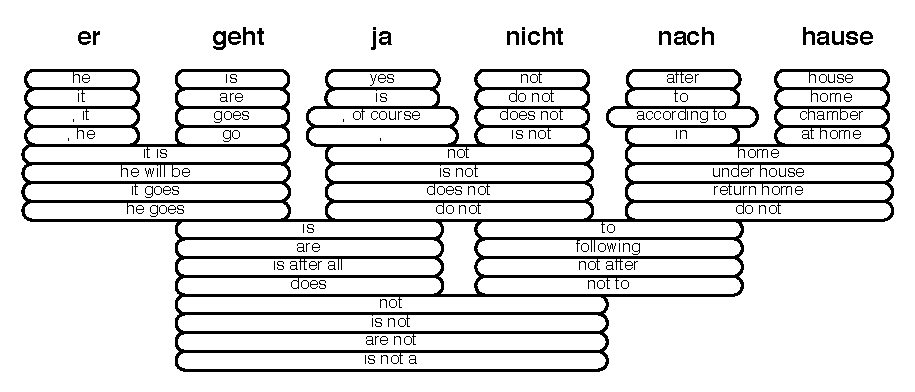
\includegraphics{g/translation-options.pdf}
 \caption{Translation Options}
 \caption*{\textit{\cite{Koehn2009a}}}
\end{figure}

This translation options are used as building blocks in a process known as \textit{hypothesis expansion}. During this process, a data structure known as \textit{search graph} is being built by sequentially joining translation options that cover different parts of sentence in source language (Figure 2.2). Nodes of this graph are called \textit{hypotheses}. As new translation options are being added to existing hypotheses, new partial translation is formed \citep{Koehn2009a}. This process continues until the sequence of hypotheses covers all parts of the input sentence. Each hypothesis contains information about the translation being attached in the current step, the total score of the current partial translation, a link to the previous hypothesis that is extended by the current one and change in the coverage vector of the foreign language sentence.

\begin{figure}
 \centering 
 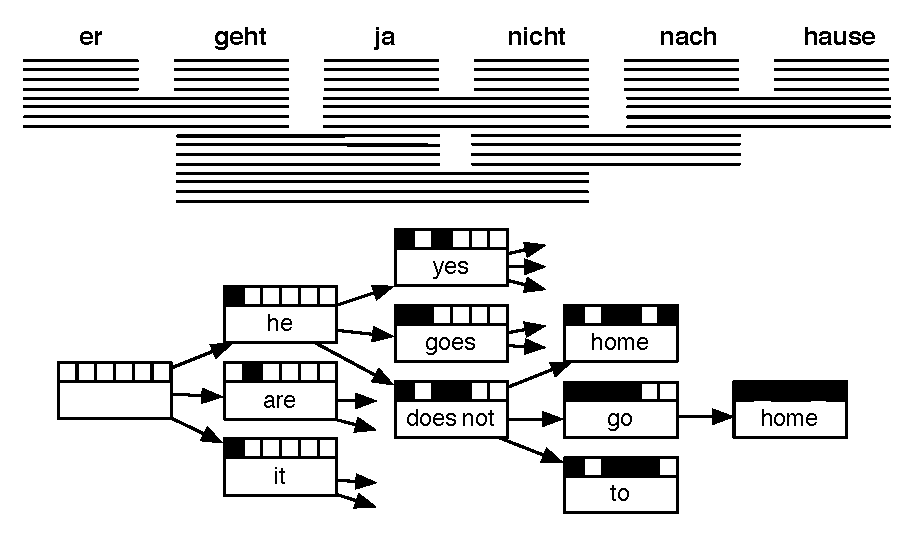
\includegraphics{g/decoding-step5.pdf}
 \caption{Hypothesis expansion}
 \caption*{\textit{\cite{Koehn2009a}}}
\end{figure}

\subsection{Hypothesis recombination}

The resulting data structure is still too large to be directly used for translation search. Several techniques are applied in order to reduce its size. One way is using \emph{hypothesis recombination}, which merges paths with same output and foreign language coverage. This reduction is risk-free and may not cause losing a good translation option. Sample recombination is illustrated on Figures 2.3 and 2.4. Both hypotheses before recombination produce the same output and cover same parts of source sentence, therefore the one with lower score could be recombined to reduce search space. Although this technique removes many unnecessary paths from graph, applying recombination does not affect overall exponential growth in number of hypothesis. 

\begin{figure}
 \centering 
 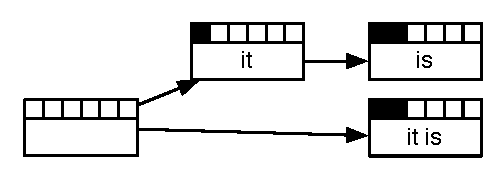
\includegraphics{g/recombination-example1.pdf}
 \caption{Before recombination}
 \caption*{\textit{\cite{Koehn2009a}}}
\end{figure}


\begin{figure}
 \centering 
 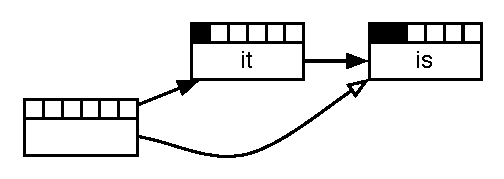
\includegraphics{g/recombination-example2.pdf}
 \caption{After recombination}
 \caption*{\textit{\cite{Koehn2009a}}}
\end{figure}


\subsection{Pruning}

Further reduction of the search graph is required for longer sentences. \textit{Stack decoding} is applied in order to filter hypothesis that have low probability of leading to good translations. Essential difference from recombination is that, this reduction technique is not risk-free and potentially may eliminate some useful translations. During this process stacks containing hypotheses with same coverage are constructed and pruning methods like histogram and threshold pruning are applied. As result number of items in stacks are reduced. 

\subsection{Summary}

In this section we provided a brief introduction into phrase-based Statistical Machine Translation, focusing on decoding stage during which search graph is being produced. Two reasons of erroneous translation produced by the process we described are \textit{search error} and \textit{model error}. While the first one corresponds to failure of finding the highest scoring translation during search, the second one refers to initial problems in the machine translation model. The assistance tool developed and investigated by us aims to help users to fix these errors within a Computer Aided Translation system by pointing to erroneous parts and selecting a better paraphrasing option from the suggestions list. In some sense our approach lets user reuse information collected during decoding. This information is available as search graph output, which optionally could be returned by Moses, together with translation results. 

\chapter{Design and implementation}

In previous chapter, we introduced Computer Aided Translation, discussing how multiple assistance ways provided within systems implementing this concept  relate to our novel tool that aims to support translators by providing an ability to fix specified parts of the translation using paraphrasing options. Furthermore, we discussed previous paraphrasing approaches highlighting similarities and difference with technique we use to search paraphrases. And finally a brief overview of phrase-based Statistical Machine Translation was provided to introduce origins of the search graph, data structure that we use as main source for paraphrasing.

Current chapter will provide detailed description of work that was carried out during this project. We start by analysing requirements for paraphrasing service within a CAT system. After that an iterational design and implementation process we applied to develop working version of such service. Major design decision that were made during the work on project will be introduced and justified. 

\section{Analysing requirements}

As mentioned earlier, an essential aspect of our paraphrasing approach is that it aims to provide a real-time targeted paraphrase search. Unlike previous efforts discussed by us before, we consider an interactive environment were queries sent by users are executed against our data model and results after being dynamically filtered and ranked using various heuristics are returned to user interface. In this section we list main requirements for our approach that were considered during design stage.

\textbf{Integration with existing CAT software}. Taking into account that most of modern CAT implementations are providing web based service (Caitra, Casmacat, MateCat), we also employed the client-server architecture to design our paraphrasing service. It might be easily attached as a module to the services provided online. Moreover, our service could also be hosted as a standalone service and integrated with desktop translation software by providing an API. This way our paraphrasing assistance might be accessible from all major types of CAT applications.

\textbf{Reusing results of machine translation}. Another important feature of our paraphrasing system is being able to produce paraphrases using only data available as a result of machine translation that provides post-editing assistance, rather requiring any additional paraphrase corpora. We designed our implementation to support translation output generated by Moses []. The process of retrieving and processing search graph will be reviewed by us in [section 3.2].

\textbf{Importance of ranking}. Quality of final ranking of the paraphrasing options is crucial requirement for RePhraser that aims to provide an interactive service. Indeed, basic concepts of Human-Computer Interaction suggest that paraphrasing options displayed to users will be efficient only in case if there count doesn't exceed 7. This means that it's important to rank top results in a way that they will contain at least one good paraphrase. Features that we exploited for ranking as well as a dynamic system of filters and sorters that we applied to improve top results will be described in [section 3.5].  


\textbf{Paraphrasing granularity}. Various levels of paraphrase granularity are studied. In case of entire sentences the task is known \textit{sentential} (or \textit{clausal}) paraphrasing, for shorter items it is called \textit{lexical} (or \textit{phrasal}) paraphrasing. For our project we investigated only lexical paraphrases, motivating this decision by the fact that other assistance tools within a CAT system may already provide multiple translation options for entire sentence, for example results of translation by using different bilingual parallel corpora. We also acknowledge that within scope of lexical paraphrases there is a further separation into two classes that correspond to shorter and longer phrases. Both cases were considered by us during evaluation stage.

We also took into account following study {[]}, which analyses usage patterns of another assistance tool, bilingual concordancer where authors suggest that average length of the input query is 2-3 words. Parallels between this assistance way and ours were discussed in previous chapter and in practice they motivate expectation of average paraphrasing query length to be similar.

\textbf{Realtime experience}. Another requirement for our interactive tool is providing paraphrasing options as fast as possible. Our tool will not be useful at all if it takes it to return results longer that time user spends on manual paraphrasing. Thus we considered time required to generate paraphrases in our evaluation. 

\textbf{Coexistence with manual editing}. While RePhraser aims to be used in order to fix erroneous part in the translation by getting the corrected paraphrase automatically, we acknowledge that final high quality translation cannot be achieved only by using paraphrasing. An ability to manually post-edit translation is crucial and designing our approach we considered that it will be used in an environment where translation could be altered by user at any time.  

\section{Preparing data}

\subsection{Retrieving search graph dump file}

A representation of the search graph, described by us in Section 2.3, could be optionally returned by Moses using \textsf{-output-search-graph FILE} parameter. Resulting text file contains list of hypotheses that were considered during the decoding stage. Each line in the file represent such hypothesis. Contents of file is ordered by sentence identifiers, that appear in the beginning of each line indicating to the sentence that was being translated when the hypothesis formed. The hypotheses are in one of three possible formats.

The \textit{initial hypothesis} refers to the empty hypothesis that is used as starting point in process of hypothesis expansion. This hypotheses have a simple structure and don't carry any additional information:

\begin{verbatim}
0 hyp=0 stack=0
\end{verbatim}

The \textit{regular hypothesis} encodes information about translation decisions that were made by the decoder in a given state. Sample regular hypothesis has following format:

\begin{verbatim}
0 hyp=10 stack=1 back=0 score=-1.497 transition=-1.497 forward=3437
fscore=-8.900 covered=0-0 out=del Parlamento
\end{verbatim}

The line starts with sentence identifier which is followed by a unique hypothesis identifier \textsf{hyp=10}. This identifier is used to reference hypotheses. The stack in which hypothesis is placed identified by \textsf{stack=1}, this is also the number of words covered in original input. The next attribute \textsf{back=0} is a reference to the previous hypothesis, in this case it refers to the initial empty hypothesis. This means that current hypothesis represents the first translation option addition. Overall score of current partial translation is expressed as \textsf{score=-1.497}, which derives from a log-probability which is calculated given machine translation models. The cost of transition to current state is available as \textsf{transition=-1.497}. After finalising the translation, hypothesis attributes are enriched by adding information about the best forward step \textsf{forward=3437} and score \textsf{fscore=-8.900} to the end of the graph. Original sentence coverage information is available in following format \textsf{covered=0-0}, where \textsf{0-0} indicates covered interval.
Finally, the last attribute \textsf{out=del Parlamento} contains the translation option that was added by introducing current hypothesis.

The third type of hypothesis groups \textit{recombined hypotheses}. That are omitted as a result of recombination process that was reviewed by us in Section 2.3.5. Recombined hypotheses have following format

\begin{verbatim}
0 hyp=734 stack=2 back=24 score=-2.684 transition=-1.226 
recombined=731 forward=8037 fscore=-7.962 covered=3-3 out=de Apoyo
\end{verbatim}

Here additional attribute \textsf{recombined=731} indicates to the hypothesis with a better score, with which current hypothesis was recombined.

Another option fetching the information generated during decoding is executing Moses with \textsf{-verbose 3} parameter. This way detailed logs will be provided by the system. The resulting output will contain mostly discarded hypotheses and will not have information about best path that is being added in case of the switch we described earlier. That is why we prefer using the \textsf{-output-search-graph} option instead.

More details are available at [http://goo.gl/6RYbDK]

\subsection{Preprocessing data for paraphrasing}

For initial testing purposes we used Moses to translate set of 3000 Russian sentences from news domain (\textit{newstest2012b}) into English. The resulting search graph dump file was about 5.7GB. In order to process it efficiently we decided to encode information from this file into a relational database. We developed a small Python script that parsed each line in the search graph file and mapped attributes into a dictionary, which was then stored in an SQLite database. The resulting transformation reduced size of our graph representation to 2.3GB. Moreover, main benefit of having our graph stored in a relational database was being able to run SQL queries against it. 

\bibliography{library}


\chapter{Evaluation}

In this chapter we provide detailed description of the evaluation process that we carried out for testing multiple versions of our paraphrasing approach. Considering the modular design of our paraphraser it was possible to design several experiments by adding and removing specific functionality. In scope of this project we were mainly interested in evaluating usefulness of paraphrasing options provided by our tool in context of a translation task. It was not feasible to set up user studies at early stage of the project, because there were too many versions to test. Considering that we designed an automatic evaluation system that helped us to find the most promising versions and also highlighted various issues and interesting features about our tool. We will begin this chapter by describing this automatic evaluation process. At the final stage of project we also carried out a small user study. We will show how results of this study supported our previous findings. Describing each evaluation stage we will also provide analysis and interpretation of the results.

\section{Automatic evaluation}

The design of our automatic evaluation is similar to the multiple translations technique that was described in the background chapter. Our main goal was to test whether our paraphraser can find a suitable paraphrase to a given part of machine translation output. To achieve this goal we created a large repository of test cases. Each test case contains a sentence corrupted by machine translation and a set of suggested paraphrases for different parts of this sentence. In our evaluation process we treat these suggested paraphrases as the gold standard. In order to collect this kind of test data, we artificially corrupted 1000 English (natural language) sentences from news domain (\emph{newstest2012b} dataset) by translating them into Russian and then back into English. This way the resulting English sentences were expressing the same idea as original ones. However, most of them were stylistically or grammatically incorrect. We detected different parts in original and corrupted version and passed the corrupted parts to our paraphraser. We considered the test case successful if corresponding original part was in top $n$ paraphrasing suggestions. In our experiments we considered $n = 5$, as this is the desired number of options displayed to the user. We begin this section by providing a short overview of the test case generation process, then we will provide the evaluation results. We will conclude current section by discussing problems of this evaluation type.


\subsection{Generating test cases}

In order to generate the test cases, we used the Moses toolkit to translate 1000 English (natural language) sentences into Russian. First, we generated a translation model for English - Russian pair using following command:

\begin{verbatim}
/moses-git2/scripts/training/filter-model-given-input.pl 
~/secondfilter ~/m2config.ini ~/eng.orig.result.in 
-Binarizer "/moses-git2/bin/processPhraseTable"
\end{verbatim} 

Then we used the generated model output (\texttt{secondfilter}) to translate sentences executing following command:

\begin{verbatim}
/moses-git2/bin/moses.2013-01-26 -mbr -mp -search-algorithm 1 
-cube-pruning-pop-limit 5000 -s 5000 -threads 24  -ttable-limit 100
-max-trans-opt-per-coverage 100 -f ~/finalfilter/moses.ini 
< /fs/vali1/wmt13-en-ru/evaluation/newstest2013.input.lc.1 > ~/rus_out_1
\end{verbatim} 

Figure 4.1 illustrates sample original English sentence (a) and it's Russian translation (b). We used a simple Python script to remove coverage information from the results in order to use it as input for Russian - English translation, sample result is illustrated on Figure 4.1 (c). Following command was used to build Russian to English translation model:

\begin{verbatim}
/moses-git2/scripts/training/filter-model-given-input.pl 
~/secondfilter ~/m2config.ini ~/rus.result.in 
-Binarizer "/moses-git2/bin/processPhraseTable"
\end{verbatim} 

Finally, we translated Russian sentences back to English by running Moses with following configurations:

\begin{verbatim}
/moses-git2/bin/moses.2013-01-26 -mbr -mp -search-algorithm 
1 -cube-pruning-pop-limit 5000 -s 5000 -threads 24  -ttable-limit 100
-max-trans-opt-per-coverage 100 -f ~/secondfilter/moses.ini 
< ~/rus.result.in > ~/en_out_new2
\end{verbatim} 

The resulting English sentence is illustrated on Figure 4.1 (d). As we can see it is different from original English input. In this case the difference is in phrases ``us states'' and ``american states''. Obviously, original phrase ``american states'' is a better translation and if our paraphraser can suggest it in top 5 results we can consider that as a successful test case. 

Considering this, we extracted all differences between original English and corrupted English sentences and stored them in our test case repository. To detect corrupted parts, we used coverage information to align parts of corrupted and original English sentences. After alignment we saved pointers to different parts. For our example, ``us states'' has coverage \texttt{|5-6|}, what corresponds to 6th and 7th words in Russian translation. As we can see from Figure 4.1 (b) these words have following coverages: \texttt{|5-5|} and \texttt{|6-6|}. These coverage information points to ``american states''. Comparing this to ``us states'' we spot the difference. We applied the same procedure for all phrases in final English translation. For each sentence we merged sequential difference intervals.

As a result we collected 2139 test cases, that were used for evaluation. While we applied this technique to collect evaluation data, it can also be seen as an alternative paraphrasing approach. Indeed, most of resulting samples were paraphrase pairs. However, this paraphrasing is very expensive and time-consuming to be used within an interactive environment. 

\begin{figure}
 \centering 
 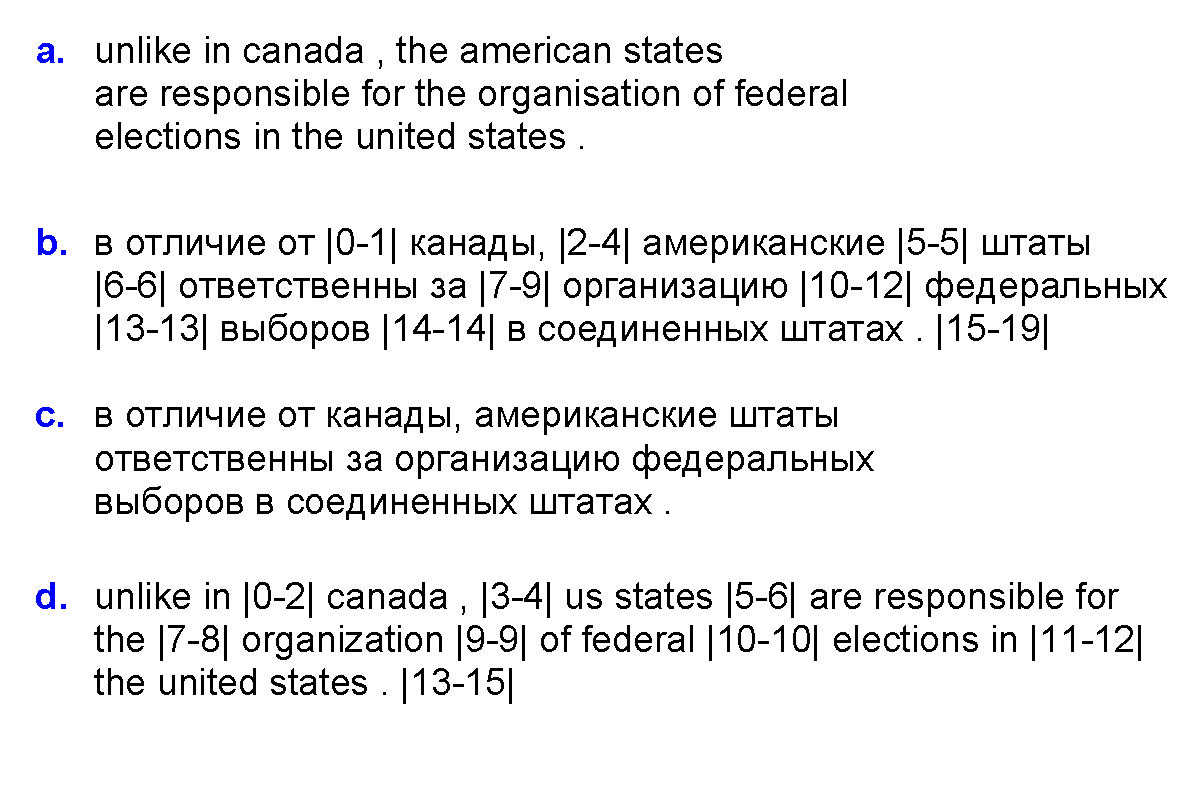
\includegraphics[scale=0.75]{g/rus-sample1.pdf}
 \caption{Resulting Russian translation}
 \caption*{\textbf{a.} The original English sentence from the \texttt{newstest2012b} dataset; \textbf{b.} The result of translation into Russian; \textbf{c.} The processed Russian translation which is used as an input for Russian to English translation; \textbf{d.} The final English translation, which is different from the original English sentence as a result of current process }
\end{figure}

\subsection{Results of automatic evaluation}

We tested ten different versions of our approach using the test case repository we discussed in previous section. These versions differ in filters, sorters and score functions. Figure 4.2 illustrates outcome of our automatic evaluation. The first columns identify types of functions we used. Description of these functions could be found in Section 3.4. The final column contains the score, which expresses the number of successfully solved test cases out of 2139 total tests.

\subsection{Analysing automatic evaluation results}

As we can see from results illustrated on Figure 4.2, we achieve the best performance with Approach 10. This approach uses all partial filters, all score functions and all sorters in same order as listed in the table. In contrast, Approach 1 has the worst performance. For this approach we did not use any filters or sorters. However we used punctuation partial filter and score difference based score function. We consider Approach 1 as the \emph{baseline} baseline approach, because it uses only minimum required functions. Furthermore, we can see that we achieve better performance by adding language model based features. Also from the results we can see that using sorters significantly improves the performance of paraphraser.


\begin{figure}
 \centering 
 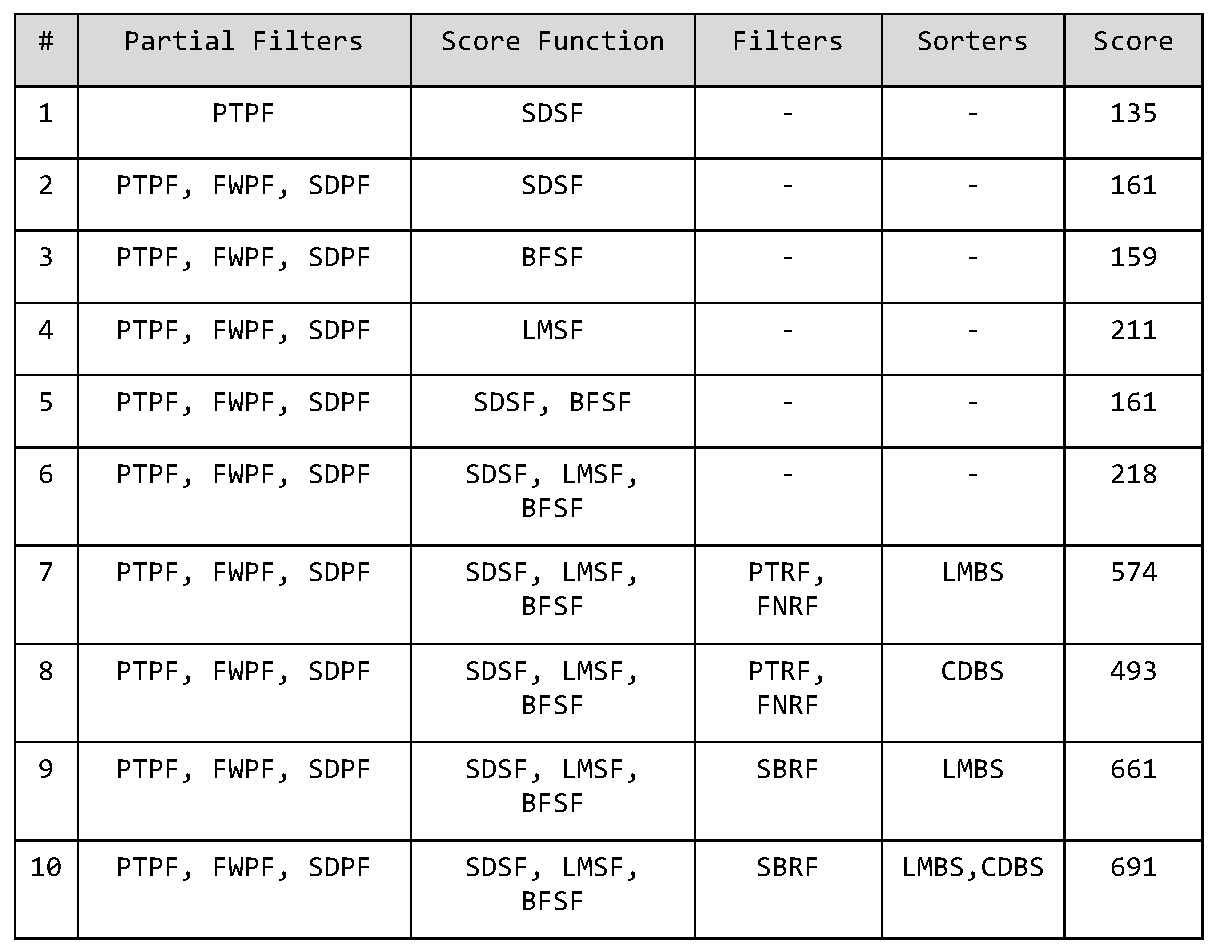
\includegraphics[scale=0.75]{g/eval-auto-results.pdf}
 \caption{Automatic evaluation results}
\end{figure}


We applied \emph{sign test} to test significance of our results. Considering $0.05$ as significance level, we found out that approaches 2 and 3 are not significantly different, as well as approaches 4 and 6. All other approaches were significantly different from each other. 

We developed a web based visualisation tool to analyse results of the automatic evaluation in greater details. This tool lists all test cases per experiment. Each item of the list is red in case of failure or green in case of success. We placed ``Details'' button in each row. Clicking this button launches a modal window which provides more details about the test case, displaying the sentence that was being translated, original paraphrasing selection, desired result and list of suggested paraphrases. This tool was implemented using JavaScript and is currently available on the project website. 

Using the visualisation tool we detected multiple problems associated with automatic paraphrases evaluation. Firstly, we noticed that our paraphraser performs significantly better in case of shorter phrases, while for longer phrases it almost always fails to find the desired paraphrase. This dependency is illustrated in Figure 4.3. However, analysing long phrases we noticed that some of them represent good paraphrasing candidates, while they do not match the original natural language English phrases. This results should be considered as success cases for paraphraser, but due to mismatch with original phrase they are classified as failure cases. If a paraphrase doesn't match the original text, it shouldn't mean a failure, it still can be a good paraphrasing option. Considering this fact our evaluation scores should be interpreted as \emph{at least} $N$ correct cases out of 2139. In order, to verify results achieved by our automatic evaluation approach we decided to carry out a user study, which will be described in the next section.

\begin{figure}
 \centering 
 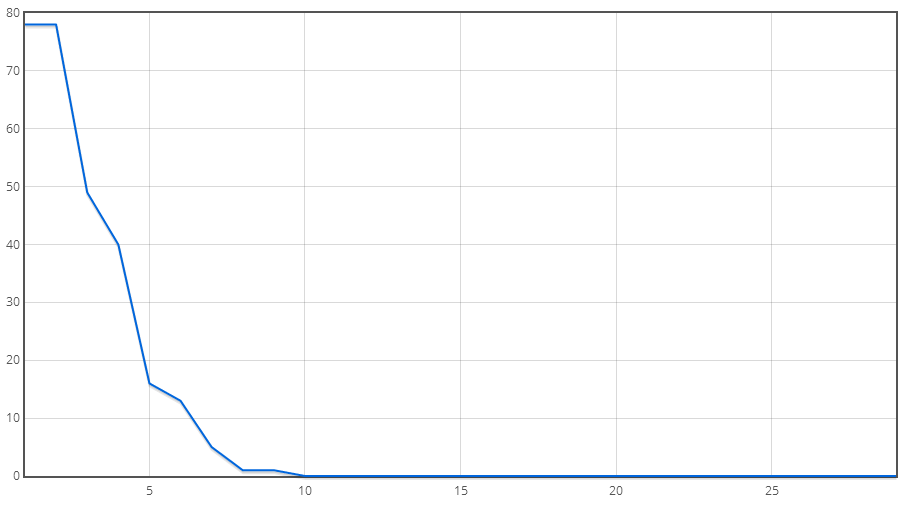
\includegraphics[scale=0.6]{g/phrase-size-chart.png}
 \caption{Relation between phrase size and paraphrasing performance}
 \caption*{X axis: number of words in phrase, Y axis: percentage of successful cases}
\end{figure}


\section{Manual evaluation}

During this project we also developed a web based interactive evaluation tool. This tool provides a user with an interface for manual evaluation of paraphrasing results. It reuses automatic evaluation test cases, displaying machine translation of the sentence. The tool also highlights an area that is considered to be corrupted as a result of alignment with original English sentences. Below the sentence we located top 5 selectable paraphrasing options that were returned by a given paraphraser version. User can pick one of these options as a better paraphrase or leave original. We also added an option for user to suggest a better paraphrase if neither options nor original text are suitable translations. Figure 4.4 illustrates the interface of our interactive evaluation tool. 

One of our goals was to make this tool easily adaptable for all paraphrasing result data we collected during automatic evaluation. To achieve this we developed a generic interface using JavaScript templating engine Handlebars.js. The data we collected during automatic evaluation stage was stored in JSON-based format and was easily rendered with our JavaScript templates.

\begin{figure}
 \centering 
 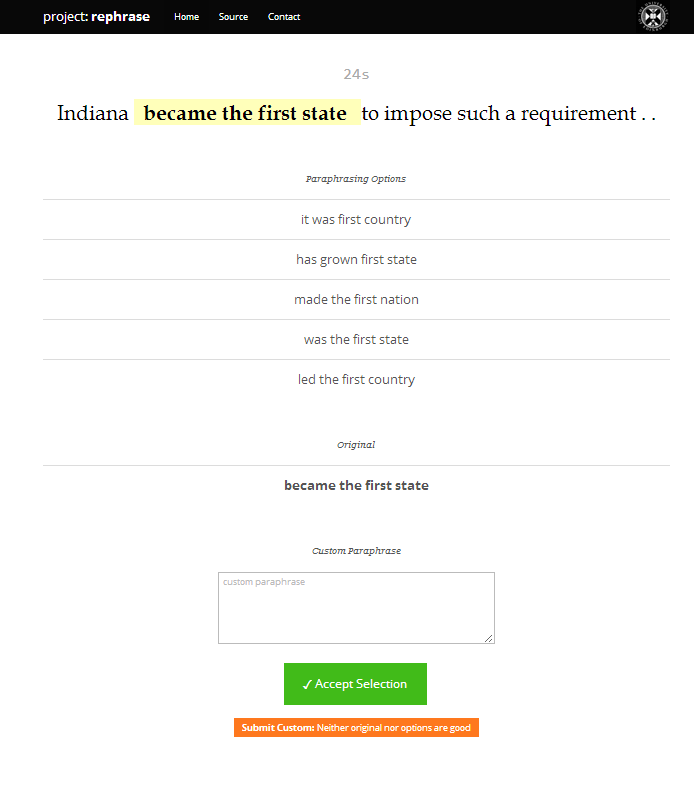
\includegraphics[scale=0.8]{g/man-eval.png}
 \caption{Manual evaluation tool}
\end{figure}

\subsection{Manual evaluation methodology}

Considering results of the automatic evaluation, we picked three out of ten tested approaches for the user study. These approaches are 1, 7 and 10. We randomly picked 50 out of our 2139 test cases, ensuring that both short and long phrases present in the final selection. We had four volunteer participants who were provided with a background information about the context of paraphrasing, they were instructed to pick a better paraphrase for selected part of sentence and to press ``Accept'', or alternatively to suggest a custom paraphrase and proceed by clicking ``Submit Custom''. 

All participants were encoded by their initials in the following way: \texttt{HG}, \texttt{OM}, \texttt{NH} and \texttt{RM}. For each of the three approaches each participant submitted his decisions for the same 50 test cases. We also considered the case when user comes across a test case that he already assessed for previous approach and his desired paraphrase selection already is in top 5 for current approaches. We automatically skipped this test cases, considering them successful. 

\begin{figure}
 \centering 
 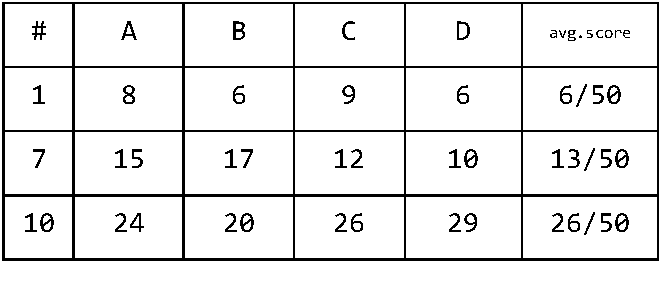
\includegraphics[scale=0.8]{g/man-eval-result.pdf}
 \caption{Manual evaluation tool}
\end{figure}

\subsection{Analysing manual evaluation results}

Final results of the user study are provided on Figure 4.5. Here the first column is approach number, four next columns contain number of successful test cases for each user. And finally last column is a unified score, which considers case successful if at least two of four annotators decided that top 5 list contains a suitable paraphrase. We can see that these results correlate with results of automatic evaluation. Indeed, applying \emph{sign test} with $0.05$ as significance level we verified that all three approaches are significantly different and most importantly that Approach 10 is significantly better than the baseline approach.

\chapter{Interactive Paraphrasing}

Earlier we highlighted that during current project we considered paraphrasing as an interactive process. We considered interests of the end user by ensuring a real-time performance as well as by focusing on ranking for top paraphrasing candidates. In this chapter we introduce further work in this direction carried out by us during the project. We tweaked our interactive evaluation tool by adding UI elements that could be used to provide quick feedback on results. This feedback is instantly handled by our system in order to produce improved results. We also modified our automatic evaluation system in order to assess usability of this new feature.

\section{Handling user feedback}

Describing paraphrasing process, we introduced a method that uses a finite state machine to output a large number of paraphrasing suggestions. However, on the next steps this list is being filtered, sorted and only top 5 results are displayed to the user. All other paraphrasing options are wasted. Considering an interactive environment, we decided to introduce a UI feature that would let user to redefine his original query in light of the results he receives from the system. Receiving this feedback we go back to the output list and reorder it considering the feedback 

Inspired by relevance feedback concept from Information Retrieval field, we added buttons labeled ``Show More Like This'' near each paraphrase option in output screen. Clicking one of these buttons initiates a server request asking to update results by biasing them towards the corresponding paraphrase candidate. Figure 5.1 illustrates the updated UI. 

\begin{figure}
 \centering 
 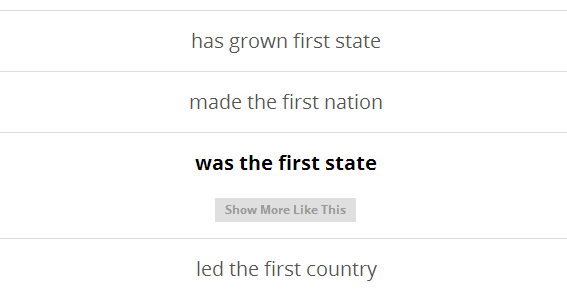
\includegraphics[scale=0.8]{g/show-more-like-this.png}
 \caption{``Show More Like This'' button}
\end{figure}

To implement this feature on the server-side, we simply developed a new sorter function, named \textbf{User Feedback Based Sorter} (\texttt{\textbf{UFBS}}). This sorter reorders final paraphrasing options list using string distance and word distance features as the primary and secondary weight functions. As a result, top items of the final are the most similar ones to the phrase specified in user feedback. 

In current implementation we re-run original query to retrieve the paraphrases list for feedback based sorting. However it's possible to implement this functionality in a more efficient way by saving results in cache, reusing them when user provides feedback. 

\section{Evaluation}

We modified our automatic evaluation process, by considering not only the original top results, but also results retrieved by providing each of the original paraphrasing option as user feedback. This way the number of potential paraphrasing candidates dramatically increased. For our baseline approach we got \textbf{501} out of 2139 matches with desired paraphrase. Our best performing approach scored \textbf{847} out of 2139 test cases. For comparison, without feedback handling feature these numbers are correspondingly \textbf{135} out of 2139 for the baseline approach and \textbf{691} out of 2139 for the best approach.

However, the automatic evaluation considers that user will always provide useful feedback, which is not a realistic assumption. To test feasibility of the new feature, we carried out another small user study. Two participants were marking 30 same test cases using an updated version of our interactive evaluation tool. For baseline approach we got \textbf{11} cases in which at least one user found the desired paraphrase and \textbf{6} cases where both users found a suitable option. For the best approach these numbers are correspondingly \textbf{23} and \textbf{18}. Sign test confirmed significance of these results. Considering this outcome and comments from the users, we conclude that the user feedback feature is really helpful in context of paraphrasing task.

\section{Specified paraphrasing requests}

Analysing the situations in which translator may want to use our paraphrasing tool, we found three core use cases:

\begin{itemize}
    \item User tries to find better wording for translation and wants to explore all options that express same meaning
    \item User expects to get a fixed version of an erroneous part in the translation
    \item User is not familiar with source language and machine translation does not seem to be good. Paraphrasing is used to understand what the selected part of translation means  
\end{itemize}

Furthermore, investigating each case in detail, we noticed that there are some other special cases when paraphrasing could be useful including:

\begin{itemize}
    \item Paraphrasing could be used to expand or collapse abbreviations. As we consider context of translation during paraphrasing this might be useful to find out correct meaning of a given abbreviation.

    \item Paraphrasing could be used to find out synonyms to a selected words in the translation. This is the main reason behind single word selection requests

    \item User might want to express same idea in a shorter or longer way, using more or less generic words. 
\end{itemize}

Considering all these situations, we designed another way of adding interactivity to our paraphrasing tool. This is done by introducing a smart ``Paraphrase'' button, which allows users to specify the main motivation behind their paraphrasing request. The button is implemented using a GUI component known as \emph{split button}, which represents a button with an arrow on the right side. Clicking the button will request default paraphrasing lookup. While clicking the arrow, will suggest more specific options based on the selection. Some use cases of the button are illustrated in Figure 5.2.   

\begin{figure}
 \centering 
 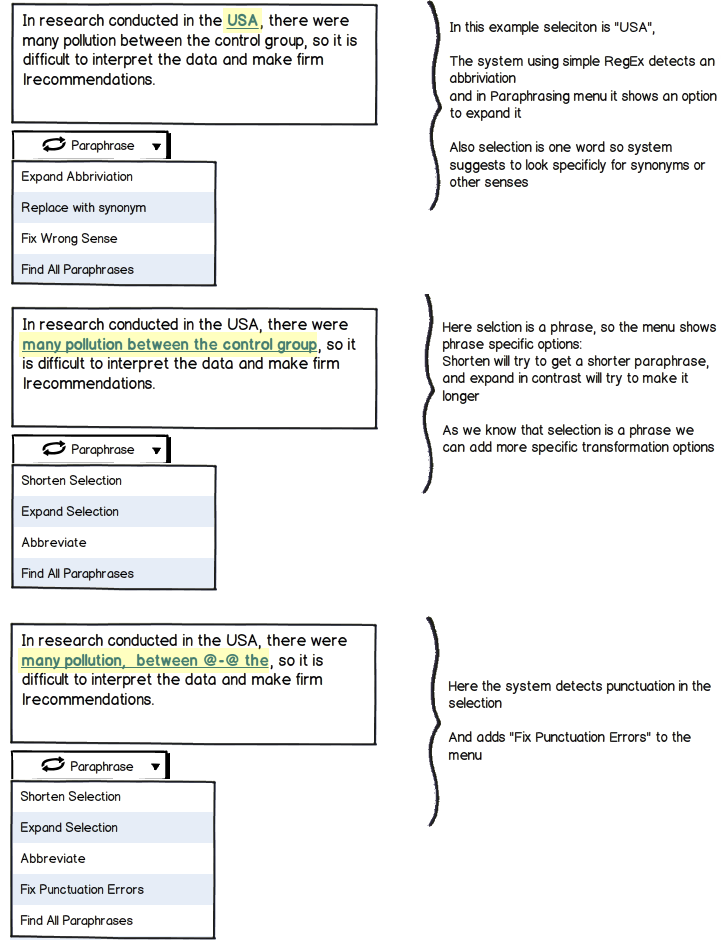
\includegraphics[scale=0.8]{g/button.png}
 \caption{``Paraphrase'' button}
\end{figure}

Similarly to user feedback functionality, these kind of specified queries are handled by introducing additional filters and sorters. In scope of this project we implemented only the ``expand abbreviation'' functionality as proof of the concept. The feature is supported by a filter that removes items where the first letters of each word doesn't follow the letters in original selection.


\chapter{Conclusion}

\section{Summary}

During this project we developed and evaluated a paraphrasing tool that could be used in process of a computer aided translation. We started by analysing state of the art assistance techniques that are available in recent CAT implementations. Trying to relate these techniques to our approach we noticed that paraphrasing task could be efficiently solved using data produced by post-editing and interactive translation assistance types. We continued our investigation by studying existing efforts in data-driven paraphrasing. We found out that paraphrasing approach that uses bilingual parallel corpora as data source [] has same high level idea as our solution. This idea is that if multiple items have same translation in foreign language, they are probably paraphrases. In contrast with previous studies, we exploited search graph data as our main source for paraphrasing. This data is being generated during decoding stage of the machine translation process.

We designed a simple paraphrasing service, which aims to find top paraphrases for user input. In Chapter 3 we described the preprocessing step which was carried out by us in order to boost graph querying performance. Next we discussed importance of coverage information and how user input is being aligned with foreign sentence. We reviewed the process of graph querying, by introducing the problem of coverage splitting and a solution we found to resolve it. Finally, our core idea was constructing a finite state machine using partial paraphrases retrieved from search graph and reduced using partial filters. This finite state machine is used to generate best paraphrasing paraphrasing options by using score functions to calculate transition scores between states. Finally, results are cleaned up using a set of filters and final ranking is produced by applying set of sorters. We implemented partial filters, score functions, filters and sorters as dynamically attachable functions. As a result our core implementation represents a framework that could easily be extended and modified. 

To test feasibility of our paraphraser we generated a large test case repository using machine translation corrupted sentences. In Chapter 4 we presented results of this automatic evaluation process for ten different versions of our paraphraser. We also commented on problems with this evaluation approach. Furthermore, we carried out a user study to confirm our previous results. The final outcome demonstrated that our best approach is significantly better that baseline approach which simply produces translation options without applying any sorters or filters.

Finally, in Chapter 5 we introduced additional features that aim to provide better paraphrasing service by taking advantage of the interactive environment. We described our implementation of a feature that allows to instantly update results based on user feedback. Moreover, we discussed various situations in which paraphrasing tool might be useful and introduced a feature that lets users to request more specific paraphrasing.

In conclusion, we demonstrated how paraphrasing could be efficiently implemented within a computer assisted translation system, by reusing data generated during machine translation. 

\section{Future work}

One of the main outcomes of this work is the modular design of paraphraser, which allows to re-implement any part of the paraphrasing process. We previously demonstrated how new features like user feedback and specified requests handling could be easily supported by introducing new filters and sorters. Considering this we believe that our approach can be used as a core for more novel types of paraphrasing. Another direction for future work is collecting paraphrasing usage logs and investigating possibility of using them as training data to improve machine translation. Finally, it might be feasible to extend our approach to support data sources other than search graph, this way it will be possible to consider paraphrasing outside of translation context.  
%% ... etc ...

%%%%%%%%
%% Any appendices should go here. The appendix files should look just like the
%% chapter files.
\appendix
\include{appendix1}
%% ... etc...


\bibliographystyle{apalike}
% \singlespace

\bibliography{library}

\end{document}
